\documentclass[12pt,letterpaper,boxed]{maths_v5}
% set 1-inch margins in the documentx
\usepackage[margin=0.9in]{geometry}
\usepackage[utf8]{inputenc} 
\usepackage[english]{babel}
% include this if you want to import graphics files with /includegraphics
\usepackage{graphicx}
\usepackage{amsmath}  
\usepackage{amsthm, thmtools}
\usepackage{braket} 
\usepackage{relsize}
\usepackage{float}
\usepackage{lmodern} % math, rm, ss, tt
\usepackage[T1]{fontenc}
\usepackage{fancyhdr}
\usepackage[dvipsnames]{xcolor}
\usepackage{framed}
\usepackage[normalem]{ulem}
\usepackage{tikz-cd}
\usepackage{tikz}
\usepackage[most]{tcolorbox}
\usepackage{bm}
%new commands
\newcommand{\normal}{\unlhd}
\newcommand{\im}{\mbox{Im}}
\newcommand{\nat}{\mbox{Nat}}
\newcommand{\ZZ}{\mathbb{Z}}
\newcommand{\RR}{\mathbb{R}}
\newcommand{\NN}{\mathbb{N}}
\newcommand{\zz}{\mathbb{Z}}
\newcommand{\rr}{\mathbb{R}}
\newcommand{\nn}{\mathbb{N}}
\newcommand{\qq}{\mathbb{Q}}
\newcommand{\dom}{\mbox{Dom}}
\newcommand{\cod}{\mbox{Cod}}
\newcommand{\id}{\mbox{id}}
%renewed commands
\renewcommand{\labelenumi}{{\bf (\alph{enumi})}} 
\linespread{1.15} 
\theoremstyle{definition}
\newtheorem{theorem}{Theorem}[section]
\newtheorem{proposition}[theorem]{Proposition}
\newtheorem{corollary}[theorem]{Corollary}
\newtheorem{lemma}[theorem]{Lemma}
% \newtheorem{definition}[theorem]{\textcolor{Plum}{Definition}}

\declaretheoremstyle[
  headfont=\color{Plum}\normalfont\bfseries,
]{colored}

\declaretheorem[
  style=colored,
  name=Definition,
  sibling=theorem
]{defn}

\declaretheorem[
  sibling=theorem,
  style=colored,
  name=Proposition,
]{prop}

\begin{document}
\section*{Differential Geometry}
\tableofcontents

\setcounter{section}{0}

\newpage
\section{Curves.}

\subsection{Parameterizations and Regular Curves}
Differential geometry mainly concerns itself with higher dimension surfaces, or manifolds, 
although here we'll look at curves. We start with curves as a way to build 
up to the study of surfaces. 

But first, what's the difference between a 
curve and a surface? Intuitively, the difference is obvious, but 
from the perspective of an alien from another dimension, it's not so obvious. 
Saying "a curve looks like a screwed up line, while a surface is like 
a bent piece of paper" would not suffice for such an alien. 
What would suffice, is the following. 

\begin{defn}
    A \textbf{curve} is a continuous mapping $f:[0, 1] \to X$, 
    where $X$ is a topological space.
\end{defn}
\begin{minipage}{0.3\textwidth}
    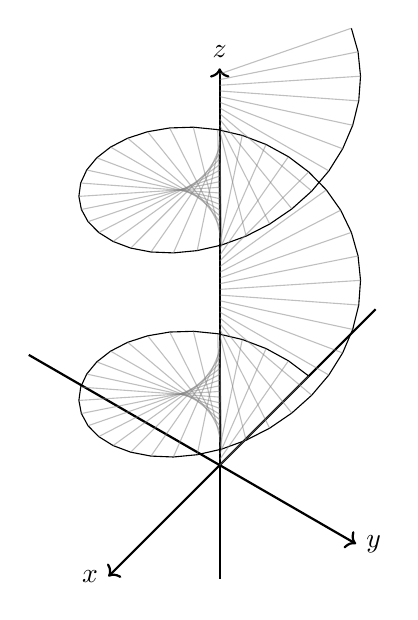
\begin{tikzpicture}[x={(0.707cm,0.707cm)},z={(0cm,0.9cm)},y={(-0.866cm,0.5cm)}, scale =0.8]
        \draw[thick, ->] (3.5,0,0) -- (-2.5,0,0) node[left] {$x$};
        \draw[thick, ->] (0,3.5,0) -- (0,-2.5,0) node[right] {$y$};
        \draw[thick, ->] (0,0,-2) -- (0,0,7) node[above] {$z$};
        \draw (1,0,0)
        \foreach \z in {0,0.1,...,7}
        { -- ({2*cos(100*\z)},{2*sin(100*\z)},{\z})
        };
        \foreach \z in {0,0.1,...,7}
        { \draw[opacity=0.5,gray] ({2*cos(100*\z)},{2*sin(100*\z)},{\z}) -- (0,0,\z);
        }
        \end{tikzpicture}    
\end{minipage}
\begin{minipage}{0.6\textwidth}
    \textcolor{MidnightBlue}{The reason why we use the interval $[0, 1]$ is because 
    we can always rescale our domain to simply be the unit interval. 
    That's what makes curves nice.} Thus the difference between a 
    curve and a surface is \textit{where} they come from; a curve is from 
    some interval, while a surface is from a subset of $\rr^2$. This is somewhat an 
    oversimplification, and we could offer even nicer defintions for a curve; one could 
    consider it to be a 1-manifold. 
    \\

    The above definition will suffice, since we will mainly be considering 
    when $X = \rr^3$; an example of such a curve is on the left, which is 
    simply a helix with parameterization
    \[
        x(t) = \cos(t) \quad y(t) = \sin(t) \quad z(t) = t.
    \]
\end{minipage}
\vspace{1cm}
\begin{defn}
    A \textbf{parameterized, differentiable curve} is a differentiable 
    mapping $f: I \to \mathbb{R}^3$, where $I$ is an open subset of $\rr$. 
\end{defn}
The above illustration is such an example, since we can differenitate the curve 
very nicely: 
\[
    x'(t) = -\sin(t) \quad y'(t) = \cos(t) \quad z'(t) = 1. 
\]
\textcolor{MidnightBlue}{Note that we cannot work off of the previous definition of a 
curve since we now need to guarantee that $X$ is a metric space 
in order to use a concept such as differenitability. The previous definition 
was simply meant to demonstrate the essence of a curve.}

So, why do we now want our curve to be differentiable? The idea of 
differentiable geometry is to extract information from the geometry of data, 
and the first step in that direction involves examining the derivative. 
To do that, it needs to first exist. For example, if we
have a curve $\alpha(t) =  (x(t), y(t), z(t))$, 
knowledge of the derivative $\alpha'(t)$
gives rise to the classic arc length formula $s(t)$ for a curve.
\[
    s(t) = \int_0^{1}\sqrt{(x'(t)^2 + y'(t)^2 + z'(t)^2)}dt = \int_0^{1}|\alpha'(t)|dt. 
\]
Having the derivative also allows us to \textbf{parameterize with respect 
to arc length}. Such a parameterization is extremely useful. While there 
are a number of ways to say "at $t=$blah, where am I?" such a parameterization 
says "when my \textit{arc length} is, say, 1, where am I?" 

Specifically, what we can do is compute $s(t)$ and solve for $t = t(s)$. 
Then, $\alpha(t(s))$ is our same curve, but this time parameterized with 
respect to arc length. Then we see that 
\[
    \left|\frac{d(\alpha(t(s)))}{ds}  \right|
    = 
    \left| \frac{d(\alpha(t(s)))}{dt} \cdot \frac{dt}{ds} \right|
    = 
    \left| \frac{d(\alpha(t(s)))}{dt} \cdot \frac{1}{\alpha'(t)} \right|
    = 1
\]
if $\alpha'(t) \ne 0$. This is really nice! If we imagine the 
derivative as a tangent vector, then this says such a vector has unit length.
This then motivates the 
following definition.

\begin{defn}
    A parameterized, differentiable curve $\alpha: I \to \rr^3$ 
    is \textbf{regular} if $\alpha'(t) \ne 0$ for $t \in I$. 
\end{defn}

If you imagine such a curve as a particle moving in three dimensional space, 
it would have to be one which doesn't stop moving (i.e., its 
velocity is nonzero at all points). 

\newpage
\subsection{Fundamental Theorem of Curves}
For this section, we'll continue to consider differentiable curves 
$\alpha(s): I \to \rr^3$ which are parameterized with respect to 
arc length. The goal will be to sort of inductively construct a 
coordinate frame which is accessible due to parameterizations 
by arc length.

Now consider the derivative of $\alpha'(s)$, which is just $\alpha''(s)$. 
Given a sufficiently smooth curve which allows a second derivative, what does 
this quantity represent? Since $|\alpha'(s)| = 1$, observe that 
\[
    |\alpha'(s)| = 1 
    \implies 
    \alpha'(s)\cdot \alpha'(s) = 1
    \implies 
    2\alpha''(s)\cdot\alpha'(s) = 0 
    \implies 
    \alpha''(s)\cdot \alpha'(s) = 0.
\]
\textcolor{MidnightBlue}{This is a common technique in differential 
geometry. If you don't know where to start with something, just 
take the derivative and see what happens!}

Hence $\alpha''(s)$ is a vector which is orthogonal to $\alpha'(s)$. 
Moreover, the fact that $|\alpha'(s)| = 1$ implies that $|\alpha''(s)|$ simply 
records the rate at which the tangent vector \textit{changes direction}.
This motivates the follow definition.

\begin{defn}
    If $\alpha(s): I \to \rr^3$ is parameterized by arc length, then we 
    define $k(s) = |\alpha''(s)|$ to be the \textbf{curvature} at $s$. 
    In this case $k(s): I \to \rr_{\ge 0}$. 
\end{defn}

Again, the function $k(s)$ measures how \textit{quickly} 
the tangent vector is changing direction. In addition, since $\alpha''(s)$ 
and $\alpha'(s)$ form a orthogonal pair, we make the next following definition.
From here on, we'll denote $\alpha'(s) = \bm{t}(s)$. 

\begin{defn}
    if $\alpha(s): I \to \rr^3$ is parameterized by arc length, we 
    define the unit vector $\bm{n}(s) = \dfrac{\alpha''(s)}{||\alpha''(s)||}$ 
    to be the \textbf{normal vector}. 
    Since $\bm{t}(s)$ and $\bm{n}(s)$ therefore form an \textit{orthonormal} pair for 
    each $s$, we define the plane containing the two vectors to be 
    the \textbf{osculating plane}.  
\end{defn}

Note that for these definitions to hold, we need $k(s) \ne 0$. Thus we'll 
assume that such is the case going forward. Finally, we finish our construction 
by considering a vector orthogonal to our osculating plane. 

\begin{defn}
    Given an osculating plane generated by $\bm{t}(s)$ and $\bm{n}(s)$ on a 
    curve $\alpha(s)$, define the \textbf{binormal vector} $\bm{b}(s)$ as the cross 
    product $\bm{t}(s)\times \bm{n}(s)$.
\end{defn}
Note that 
\[
    ||\bm{b}(s)|| = ||\bm{t}(s) \times \bm{n}(s)|| = ||\bm{t}(s)|| \cdot ||\bm{n}(s)|| \sin(\theta) = 1
\]
where $\theta$ is the angle between $\bm{t}(s)$ and $\bm{n}(s)$, which is of course 
$\dfrac{\pi}{2}$. Therefore, the binormal vector is a unit vector. In addition, we have that 
\[
    \bm{b}'(s) = \bm{t}'(s) \times \bm{n}(s) + \bm{t}\times \bm{n}'(s) 
    = 
    \bm{t}\times \bm{n}'(s).
\]  
Hence we see that $\bm{b}'(s)$ and $\bm{t}$ are orthogonal, so 
$\bm{b}'(s)$ is parallel to $\bm{n}$. Hence we see that 
\[
    \bm{b}'(s) = \tau(s)\bm{n}(s)
\]
for some function $\tau(s): I \to \rr$. This is generally referred to as the 
\textbf{torsion} of $\alpha$ 


At this point, we have the following proposition.

\begin{prop}
    Let $\alpha(s): I \to \rr$ be a regular curve, parameterized with respect 
    to arc length, such that $\alpha''(s) \ne 0$. Then for each $s \in I$, 
    there exists an orthonormal triplet given by $\{\bm{t}(s), \bm{n}(s), \bm{b}(s)\}$, 
    generally called the \textbf{Frenet moving frame}. Moreover, we have the so-called 
    \textbf{Frenet formulas:}
    \begin{align*}
        \bm{t}'(s) &= k(s)\bm{n}\\
        \bm{n}'(s) &= -k(s)\bm{t}(s) - \tau\bm{b}\\
        \bm{b}'(s) &= \tau\bm{n}
    \end{align*}
\end{prop}

However, the converse of this result is true. 

\begin{thm}[Fundamental Theorem of Local Curves.]
    Given the functions $k(s), \tau(s): I \to \rr$, there exists a 
    regular, parameterized curve $\alpha: I \to \rr^3$ such that 
    \begin{itemize}
        \item $s$ is the arc length
        \item $k(s)$ is the curvature
        \item $\tau(s)$ is the torsion.
    \end{itemize}
    If $\overline{\alpha}$ is another regular, parameterized curve satisfying the above 
    criterion, then $\overline{\alpha}$ and $\alpha$ differ by a rigid motion.
\end{thm}
If one considers the collection of all regular, paramterized curves, and then 
mods out the space by the equivalence relation where two curves are equivalent if they 
are the same up to some rigid motion (obviously reflexive, symmetric, and transitive by composing
matrix transformations) then the above theorem says that every 
equivalence class is uniquely determined by a triple $(s, k(s), \tau(s))$. 
\textcolor{MidnightBlue}{As a result, the interpretation of such 
uniqueness on equivalence classes is that every curve is basically a straight 
line which is subjected to curvature (bending) and torsion (twisting).}


\newpage
\section{Regular Surfaces.}
\subsection{Manifolds and Regular Surfaces.}
In this section, we now move onto surfaces. In the same spirit as the previous section, 
we first narrow our surfaces of interest since we want to deal with classes 
of surfaces which are nice enough to say something general. Thus we begin with 
the concept of a manifold. 


\begin{defn}
    A $\bm{n}$\textbf{-manifold} is a separable metric space $M$ 
    which is \textbf{locally homeomorphic} to $\rr^n$. What we mean by 
    locally homeomorphic is that, for each $p \in M$, there is a neighborhood $U$ of $p$ 
    which is homeomorphic to some open set in $V$ in $\rr^n$.
    \\

    \noindent \textcolor{Red}{Alternatively}, we can define a $\bm{n}$-\textbf{manifold} to be a
    second-countable Hausdorff space $M$ which locally homeomorphic to $\rr^n$. 
\end{defn}
\textcolor{MidnightBlue}{The above defintions are nearly equivalent: a separable metric space is second countable, 
which is also 
Hausdorff since a metric space is Hausdorff. On the other hand, a second countable, Hausdorff 
space is not necessarily a separable metric space, since not every Hausdorff 
space can form a metric space (lots of weird counterexamples point this out).
In some sense, it is better to use the first definition to dodge these 
weird counterexamples, but lots of people use the second anyways.}

As a side note, it turns out that manifolds form a \textbf{category}, 
hilariously called $\textbf{Man}_{p}$. 
The objects are manifolds, and the morphisms are functions which are $p$-times 
continuously differentiable.

\begin{defn}
    Let $f: M \to N$ be a mapping between two manifolds. If $f$ is a 
    differentiable homeomorphism (that is, its inverse is also differentiable)
    then $x$ is a \textbf{diffeomorphism}. 
\end{defn}

\begin{defn}
    Let $M$ be a $n$-manifold, and suppose
    $U$ is a subset of $\rr^m$. A diffeomorphism 
    $\bm{x}: U \to M$ is said to be a \textbf{parameterization} of $M$. 
\end{defn}

\begin{example}
    Here's a simple example. The torus is of course a manifold, and a parameterization 
    of such a structure is given by 
    \[
        \bm{x}(\theta, \phi) = ((R\cos(\theta) + r)\cos(\phi), (R\cos(\theta) + r)\sin(\theta),r\sin(\theta))
    \]
    where $\phi, \theta \in [0, 2\pi]$.



\end{example}

Let's now reduce our scope and consider a special type of manifold known,
as a regular surface. 
\begin{defn}
    Let $S \subset \rr^3$ and let $p \in S$. If there exists 
    a neighborhood $V \subset \rr^3$ of $p$ and an open set $U \subset \rr^2$ 
    with a map
    \[
        \bm{x}(u, v): U \to V \cap S
    \]
    where 
    \begin{itemize}
        \item[1.] $\bm{x}(u, v)$ is diffeomorphism
        \item[3.] The differential $d\bm{x}_q:\rr^2 \to \rr^3$ is injective.
    \end{itemize}
    then $S$ is said to be a \textbf{regular surface}. Or, more easily, 
    a \textbf{regular surface} is a $2$-manifold whose inclusion mapping $S \to \rr^3$ is 
    a homeomorphic immersion.
\end{defn}
\textcolor{MidnightBlue}{So, what does this mean? This means that to be 
a regular surface, we need to be able to parameterize open sets of the 
surface using open sets from $\rr^2$. Furthermore, the differential of 
these parameterizations must behave well (which we'll see later will 
serve the purpose of allowing us to define a tangent space at each point).}



\begin{prop}
    Let $U \subset \rr^2$ be open. Suppose $f(u, v): U \to \rr$ is a
    differentiable function. Then the subset $S$ of $\rr^3$
    \[
        S = \big\{(u, v, f(u, v)) \mid u, v \in U\big\}    
    \]
    is a regular surface.
\end{prop}

\begin{prf}
    To prove this, we examine the map 
    $\bm{x}(u, v) = (u, v, f(u, v))$. First, note that $\bm{x}(U) = 
    S$, so that we have the first part of the definition of a regular surface satisfied. 
    We certainly have that $\bm{x}'(u, v)$ exists and is well defined. 
    In addition, $\bm{x}$ is clearly a continuous bijection. 
    Note that since $(u, v) \mapsto (u, v, f(u, v))$, we can define 
    \[
        \bm{x}^{-1} = \pi_2^3: \rr^3 \to \rr^2 \qquad \pi_2^3(u, v, f(u, v)) = (u, v).        
    \]
    Therefore $\bm{x}^{-1} = \pi_2^3\big|_{S}$. Since projection maps are continuous, 
    so is its restriction onto an open set. Hence $\bm{x}^{-1}$ is continuous. 

    Finally, note that if $q \in U$,
    \[
        d\bm{x}_q = 
        \begin{pmatrix}
            1 & 0\\
            0 & 1\\
            f_u & f_v 
        \end{pmatrix}.
    \]  
    As the columns are linearly independent, we see that $d\bm{x}_q$ is 
    injective. Therefore, $S$ is a regular surface.
\end{prf}
This proposition guarantees that a real valued functions in second variables, which 
are differenitable, can reliably form regular surfaces. An example of this would 
be something like a topographical map; after all, a topographical map is a three dimensional 
surface projected down into two dimensions, whose values allow us to undestand how
steep a certain hike is. In addition to this, this proposition allows us to establish a functor between the category of 
differentiable functions $f: \rr^2 \to \rr$ and the category of regular surfaces. 

\begin{defn}
    Let $f: U \to \rr^m$ be a differentiable map where $U \subset \rr^n$,
    and let $p \in U$. If $df_p: \rr^n \to \rr^m$ is not injective, then 
    we say $p \in U$ is a \textbf{critical point}, and that $f(p)$ is a 
    \textbf{critical value}. If $q \in \rr^m$ is not a critical point 
    then it is a \textbf{regular value}.
\end{defn}

\begin{prop}
    Let $f:U \to \rr$ be a differentiable function, where $U \subset \rr^3$, and suppose $a \in f(U)$ 
    is a regular value. Then $f^{-1}(a)$ is a regular surface in $\rr^3$.
\end{prop}
    
\begin{prf}
    Let $p \in f^{-1}(a)$. Then since $a$ is a regular value, we see that 
    $df_p = (f_x, f_y, f_z)$ is an injective mapping. For this to be the case, 
    we the partials $f_x, f_y, f_z$ cannot simultaneously be zero when evaluated 
    at $p$. Without loss of generality, suppose $f_z$ is nonzero. 

    Now consider the mapping $F: U \to \rr^3$ where 
    $F(x, y, z) = (x, y, f(x, y, z))$. Then we have that 
    \[
        dF_p 
        = 
        \begin{pmatrix}
            1 & 0 & 0\\
            0 & 1 & 1\\
            f_x&f_y&f_z
        \end{pmatrix}.
    \]
    Since $\det(dF_p) = f_z \ne 0$, linear algebra tells us that this mapping is 
    invertible. By the inverse function theorem, there exists open subsets 
    $V$ of $p$ and $W$ of $F(p)$ such that $F: V \to W$ is one to one, and 
    $F^{-1}:W \to V$ is differentiable. Let $F^{-1} = (u, v, g(u, v, t))$ where 
    $(u, v, t) \in W$. Then $g(u, v, t): \rr^3 \to \rr$ is differentiable, 
    and so is $h(u, v) = g(u, v, a): \rr^2 \to \rr$. However, observe that 
    \[
        F(f^{-1}(a) \cap V) = W \cap \{(u, v, a) \mid (u, v) \in \rr^2\}.
    \]
    Therefore, the graph generated by $(u, v, h(u, v))$ is $f^{-1}(a)\cap V$. 
    Thus we see that the properties of $F$ allow $f^{-1}(a)$ to be a regular surface. 
\end{prf}

\begin{prop}
    Let $S \subset \rr^3$ be a regular surface. Then for each $p \in S$, there
    exists a neighborhood $V$ of $p$ such that $V$ is the graph of a differentiable function.
\end{prop}
\textcolor{MidnightBlue}{What we mean by being a graph of a function is a 
that one of the three must be true.
\begin{align*}
    &V = \{(x, y, f(x ,y)) \mid x, y \in \rr^2\}\\
    &V = \{(x, g(x, z), z) \mid x, z \in \rr^2\}\\
    &V = \{(h(y, z), y, z) \mid y, z \in \rr^2\}
\end{align*}
where $f, g$ and $h$ are differentiable functions.}

\begin{prf}
Let $\bm{x}: U \to S$ be a parameterization of $S$. 
Then by definition, $\bm{x}$ is a diffeomorphic immersion $\bm{x}: U \to V \cap S$. 
Because $\bm{x}$ is an immersion, we know that $d\bm{x}_q$ is injective 
where $q = f^{-1}(p)$. If we write $\bm{x} = (x(u, v), y(u, v), z(u, v))$ then 
\[
    d\bm{x}_q = 
    \begin{pmatrix}
        x_u & x_v\\
        y_u & y_v\\
        z_u & z_v
    \end{pmatrix}    
\]
but injectivity of $d\bm{x}_q$ implies that the Jacobian determinants 
\[
    \frac{\partial(x, y)}{\partial(u, v)}
    \quad 
    \frac{\partial(x, z)}{\partial(u, v)}
    \quad 
    \frac{\partial(y, z)}{\partial(u, v)}
\]
cannot simultaneously be zero at $q$. Without loss of generality, suppose 
that $\dfrac{\partial(x, y)}{\partial(u, v)}(q)$ is nonzero. If we let $\pi: \rr^3 \to \rr^2$ 
be the projection map where $(x, y, z) \mapsto (x, y)$, then we see that 
$\pi \circ \bm{x}: \rr^2 \to \rr^2$; specifically, $\pi \circ \bm{x}: U \to \rr^2$. 
The punchline is we can apply the inverse function theorem to \textit{this} 
function so that there exists open subsets of $\rr^2$, $W_1$ 
of $q$ and $W_2$ of $\pi(p)$, such that 
$(\pi \circ \bm{x})^{-1}: W_2 \to W_1$ is differentiable. Now let 
$V = \bm{x}(V_1)$, so that $\pi(V) = V_2$. Then construct the map $g(u, v) = z(u, v)$. 
Then we see that 
\[
    V =   \{(x, y, g(x ,y)) \mid x, y \in \rr^2\}  
\]
so that $V$ is the graph of a differentiable function, as desired. 
\end{prf}

\newpage
\subsection{Change of Parameters and Differentiability}
In the definition of a regular surface, we basically need to collect a series 
of parameterizations $\bm{x}_i: U_i \to S$ where $U_i$ are open subsets 
of $\rr^2$. However, sometimes we can't find these parameterizations, or we 
may wonder if there are other parameterizations of the surface. That is, 
is there are  "right" way to parameterize a regular surface? 

The answer is no. 

\begin{thm}[Change of Parameters.]
    Let $S$ be a regular surface and $p$ a point on $S$. 
    Suppose we have two parameterizations of the regular surface: 
    \begin{align*}
        \bm{x}: U \to S \qquad
        \bm{y}: V \to S
    \end{align*}
    where $U, V$ are subsets of $\rr^2$ and such that $p \in \bm{x}(U)\cap\bm{y}(V) = W$. 
    Then the change of parameters 
    \[
        h = \bm{x}^{-1}\circ \bm{y}: \bm{y}^{-1}(W) \to \bm{x}^{-1}(W)
    \]
    is a diffeomorphism. 
\end{thm}
\textcolor{MidnightBlue}{The above theorem says that parameterizations of 
a regular surface are in some sense the same thing. One can pass diffeomorphically 
between them!}

\begin{prf}
    Clearly $h$ is a homeomorphism, so we just need to show $h$ and $h^{-1}$ 
    are differenitable. To do this, consider $q \in \bm{y}^{-1}(W)$ so that $h(q) \in 
    \bm{x}^{-1}(W)$. Since $\bm{x}$ is a parameterization,
    suppose it has the form $\bm{x} = (x(u, v), y(u, v), z(u, v))$ and that without 
    loss of generality
    \[
        \frac{\partial(x, y)}{\partial(u, v)}(h(q)) \ne 0. 
    \]
    To apply the inverse function theorem, we construct the map $F: U \times \rr \to \rr^3$ 
    where 
    \[
        F(u, v, t) = (x(u,v), y(u,v), z(u,v) + t).
    \]
    Therefore, $F(u, v, 0) = \bm{x}$. Note that 
    \[
        \det(dF_{h(q)})
        =
        \begin{vmatrix}
            x_u & x_v & 0 \\
            y_u & y_v & 0 \\
            z_u &z_v & 1
        \end{vmatrix}
        = 
        \frac{\partial(x, y)}{\partial(u, v)}(h(q)) \ne 0.
    \] 
    Therefore, we can apply the inverse function theorem to conclude that 
    there exists a neighborhood $N$ of $\bm{x}(h(q))$ such that $F^{-1}$ 
    exists and is differentiable. Since $N$ is open, continuity implies 
    that there exists an open set $U' \subset \rr^2$ of $q$ such that 
    $\bm{y}(U') \subset M$. Now observe that 
    \[
        h|_U = F^{-1} \circ \bm{y}|_U.
    \]
    Since $F^{-1}$ is differenitable on $\bm{y}(U)$ and $\bm{y}$ is itself
    differentiable, we can conclude that $h$ must be differenitable on $U$. But 
    since $q$ is an arbitrary point of $V$, we see that $h$ is differentiable. 
    The argument here can be dualized to show that $h^{-1}$ is differentiable, 
    so that $h$, the change of coordinates, is a diffeomorphism. 
\end{prf}

Since the specific parameterization of regular surfaces are all diffeomorphic, 
the following definition of differentiability is well-defined. 

\begin{defn}
    Let $S$ be a regular surface and let $V \subset S$ be open. 
    A function 
    \[
        f: V \to \rr  
    \]
    is said to be \textbf{differentiable} 
    at $p \in V$ if for any parameterization $\bm{x}: U \to S$, with $U \subset \rr^2$ open, 
    we have $f \circ \bm{x}: U \to \rr$ is differentiable at $\bm{x}^{-1}(p)$. 
    Hence, $f$ is \textbf{differentiable} on all of $S$ if it is differentiable 
    at all points.

    \textcolor{MidnightBlue}{We can also define differentiability between surfaces.}
    Let $S_1$ and $S_2$ be surfaces, and suppose that 
    $V_1 \subset S_1$. Then a function 
    \[
        \phi: V_1 \to S_2 
    \]
    is differentiable if for any parameterizations 
    \[
        \bm{x}_1: U_1 \to S_1 \qquad \bm{x}_2: U_2 \to S_2
    \]
    with $U_1, U_2 \subset \rr^2$, the map 
    \[
        \bm{x_2}^{-1}\circ \phi \circ \bm{x_1}: U_1 \to U_2
    \]
    is differentiable at $q = \bm{x}_1^{-1}(p)$.
\end{defn}










\end{document}